\documentclass[11pt,a4paper]{report}
\usepackage[utf8]{inputenc}
\usepackage[french]{babel}
\usepackage[T1]{fontenc}
\usepackage{amsmath}
\usepackage{amsfonts}
\usepackage{amssymb}
%\usepackage{xcolor}
\usepackage[dvipsnames]{xcolor}

\usepackage{geometry}
\geometry{hmargin=2.5cm,vmargin=1.5cm}
\usepackage{wasysym}
\usepackage{graphicx}

\author{Mathieu Sarrat}
\title{LP23 - Mécanismes de la conduction électrique dans les solides}

\makeatletter
\renewcommand{\thesection}{\@arabic\c@section}
\makeatother


\begin{document}
\maketitle

\section*{Pré-requis et objectifs}

\begin{itemize}
	\item Dynamique du point matériel.
	\item Électrocinétique. Loi d'Ohm.
	\item Statistique de Maxwell-Boltzmann, équipartition de l'énergie.
	\item Dualité onde-corpuscule, équation de Schrödinger, statistique de Fermi-Dirac.
\end{itemize}

\newpage
\section*{Introduction}

Commençons par un bref rappel au sujet de la loi d'Ohm.
\begin{itemize}
	\item Lorsqu'on applique une différence de potentiel électrique à un conducteur, un courant électrique circule. Ce phénomène s'accompagne d'un dégagement de chaleur. On constate expérimentalement une relation de proportionnalité entre la différence de potentiel et l'intensité du courant :
	\begin{equation}
		U = RI
	\end{equation}	
	formulation globale de la loi d'Ohm. Ici, $R$ désigne la résistance du conducteur, telle que pour un conducteur filiforme
	\begin{equation}
		R = \rho \frac{L}{S},
	\end{equation} 
	$\rho$ étant la résistivité du conducteur, $S$ sa section et $L$ sa longueur. \textit{La circulation d'un courant à travers une résistance implique une dissipation de l'énergie 
	sous forme thermique (l'effet Joule), d'où le dégagement de chaleur.}\\
	
	\item Localement, en un point du conducteur, l'apparition d'une densité volumique de courant traduit la rupture d'un équilibre. On constate expérimentalement l'apparition d'une densité de courant s'il existe un gradient de potentiel électrique\textit{, de concentration en porteurs de charge, de température.} Dans le cas où c'est un gradient de potentiel qui est responsable, on écrit
	\begin{equation}
		\bold{J} = \sigma \bold{E},
	\end{equation}
	où $\sigma$ désigne la conductivité électrique du conducteur, mesurée en $\text{S}/\text{m}$ (Siemens par mètre). C'est la loi d'Ohm locale, et on peut, via un calcul d'intégrales, montrer qu'elle conduit à la loi d'Ohm globale. Dans un milieu homogène et isotrope, la conductivité est un scalaire constant, réel et positif. \textbf{La loi d'Ohm ainsi présentée est une loi phénoménologique, linéaire} : il y a proportionnalité entre la cause (gradient de potentiel électrique) et sa conséquence, le transport de charge électrique (densité volumique de courant).\\
	
	\item La vie tous les jours nous enseigne que \textbf{tous les solides ne sont pas de bons conducteurs d'électricité} : c'est par exemple le cas du bois, du diamant, du verre. Ces matériaux sont qualifiés d'\textbf{isolants électriques}. Le silicium, ou encore le germanium sont quant à eux qualifiés de \textbf{semi-conducteurs} et sont utilisés dans de nombreuses applications industrielles. On peut mesurer la conductivité de tout matériau : en effet, un isolant n'est pas parfait et un courant électrique, certes faible mais non nul, peut le traverser. Une échelle de conductivité permet de classer les matériaux :
\begin{itemize}
	\item $\sigma > 10^4 \text{S}/\text{m}$ : métaux conducteurs, notamment le cuivre $\sigma = 5.8\times 10^7 \text{S}/\text{m}$;
	\item $10^{-6} \text{S}/\text{m} < \sigma < 10^4 \text{S}/\text{m}$ : semi-conducteurs;
	\item $\sigma < 10^{-6} \text{S}/\text{m}$ : isolants.\\
\end{itemize}
\end{itemize}

\textbf{Cette classification est très imprécise, et n'explique évidemment pas pourquoi tel matériau a telle conductivité}. La véritable distinction entre un métal, un semi-conducteur et un isolant \textbf{réside dans la nature du mécanisme responsable de la conduction} électrique. Cette leçon a deux objectifs :
\begin{itemize}
	\item \textbf{peut-on trouver un modèle capable d'expliquer la loi d'Ohm ?}
	\item \textbf{comment expliquer pourquoi certains matériaux solides sont isolants alors que d'autres sont conducteurs ?}\\
\end{itemize}

\newpage
\section{Modèle de Drude}

Ce modèle a été élaboré par Paul Drude en 1900, en plein développement de la mécanique statistique. Les physiciens essayaient d'expliquer comment, à partir du monde microscopique, il était possible d'expliquer les lois macroscopiques. La théorie cinétique des gaz, développée entre autres par Maxwell et Boltzmann, permet de remonter à une définition microscopique de grandeurs macroscopiques comme la pression. La récente découverte de l'électron par J.J Thomson (1897) incita Drude à appliquer la théorie cinétique à un gaz constitué d'électrons, particules chargées négativement dont un mouvement d'ensemble constitue un courant électrique.

\subsection{Hypothèses fondamentales}

Drude supposa que la conduction électrique était assurée par un gaz d'électrons libres, évoluant dans le métal. Il supposa l'existence de particules chargées positivement (la matière étant électriquement neutre), mais bien plus lourdes que les électrons et donc ne participant pas à la conduction de l'électricité (le noyau atomique ne sera découvert que bien plus tard en 1911, par Rutherford, Marsden et Geiger).\\
 
Le modèle de Drude repose sur un ensemble d'hypothèses que nous allons lister :
\begin{itemize}
	\item \textbf{approximation des électrons indépendants} : on néglige l'interaction électromagnétique entre deux électrons,
	\item \textbf{approximation des électrons libres} : on néglige l'interaction électromagnétique entre un électron et un ion. Rigoureusement parlant, l'interaction entre ions et électrons n'est pas totalement ignorée : on suppose implicitement que les électrons restent contenus dans le métal, confinement qui ne peut être réalisé que grâce aux ions.
	\item un électron subit des \textbf{collisions ponctuelles avec les ions} du réseau : c'est ce processus, qui \textbf{selon Drude, est à l'origine de la résistivité des métaux.} 
	\item les électrons établissent un \textbf{équilibre thermique local} entre eux, par collisions (c'est le seul mécanisme restant) : après une telle collision, l'électron émerge avec une vitesse indépendante de celle qu'il avait avant collision, mais dont la direction est aléatoire et la norme compatible avec la température locale.\\
\end{itemize}

En d'autres termes, on suppose \textbf{un gaz parfait d'électrons}.

\subsection{Modèle de conductivité électrique}

Entre deux collisions, et en l'absence de champ électrique appliqué, les électrons se déplacent en ligne droite. Considérons un élément de volume $d\mathcal{V}$ de taille mésoscopique, contenant suffisamment d'électrons pour que le calcul des valeurs moyennes des grandeurs locales ait du sens. Localement, l'équilibre thermique des électrons est assuré, le problème est isotrope : il y a autant d'électrons allant d'un côté avec une vitesse donnée que d'électrons allant dans le sens opposé avec la même vitesse. La vitesse moyenne de l'ensemble des électrons de l'élément de volume est donc nulle.\\

Lorsqu'un champ électrique est appliqué (par exemple résultant d'une différence de potentiel appliquée en deux points du métal), les électrons sont accélérés par la force électrique et l'isotropie du gaz d'électrons est brisée. Quelle est la vitesse moyenne $\langle\bold{p}\rangle$ d'un électron de charge $q$ et de masse $m$ dans $d\mathcal{V}$ ? On supposera un champ électrique stationnaire pour simplifier le calcul, mais le raisonnement est applicable avec un champ variable.\\
	
Soit une $dt$ qui tend vers 0. Si un électron subit une collision, sa vitesse à l'instant $t + dt$ sera
\begin{equation}
	\bold{v}(t+dt) = \bold{v}' + q\frac{\bold{E}}{m}dt + O(dt^2),
\end{equation}
où $\bold{v}'$ désigne sa vitesse (tirée aléatoirement) après collision. Après collision, l'électron est accéléré par le champ électrique sur une durée $dt$.\\

Si l'électron ne subit pas de collision,
\begin{equation}
	\bold{v}(t+dt) = \bold{v}(t) + q\frac{\bold{E}}{m}dt + O(dt^2).\\
\end{equation}

\textbf{La probabilité d'une collision électron-ion pendant une durée $dt$} est donnée par
\begin{equation}
	\frac{dt}{\tau},
\end{equation}
où $\tau$ est un \textbf{temps de relaxation} ou encore \textbf{temps de collision}. En moyenne, un électron subira une collision avec un ion tous les $\tau$.\\

Entre $t$ et $t+dt$ (avec $dt < \tau $), une fraction $dt/\tau$ des électrons a subi une collision, et la fraction $(1 - dt/\tau)$ non. On en déduit la vitesse moyenne d'un électron dans $d\mathcal{V}$
\begin{equation}
	\langle\bold{v}(t+dt)\rangle = \frac{dt}{\tau} \left[\langle\bold{v}'\rangle + q\frac{\bold{E}}{m}dt + O(dt^2)\right] 
	+ \left(1 - \frac{dt}{\tau}\right) \left[\langle\bold{v}(t)\rangle + q\frac{\bold{E}}{m}dt + O(dt^2)\right],
\end{equation}
et $\langle\bold{v}'\rangle = \bold{0}$ du fait de l'équilibre thermique local : toutes les orientations du vecteur vitesse sont équiprobables après une collision.\\

En \textbf{négligeant les termes d'ordre 2 en $dt$}, on obtient
\begin{equation}
	\boxed{\frac{d}{dt}\langle\bold{v}\rangle + \frac{\langle\bold{v}\rangle}{\tau} =  q\frac{\bold{E}}{m}},
	\label{eq:Drude}
\end{equation}
une équation différentielle d'ordre 1 dont la solution est
\begin{equation}
	\bold{v}(t) = \bold{K}\text{exp}\left(-\frac{t}{\tau}\right) + \frac{q\tau}{m}\bold{E}
\end{equation}
où $\tau$ apparait comme le temps caractéristique d'un régime transitoire : $\tau$ caractérise la durée au bout de laquelle la vitesse moyenne des électrons tend vers 0 en régime libre, et aussi leur rapidité à répondre à une nouvelle sollicitation électrique.\\ 

L'équation \eqref{eq:Drude} peut s'interpréter à la lumière du principe fondamental de la dynamique appliqué à une particule fluide de volume $d\mathcal{V}$ constitutive du gaz d'électrons. Tout se passe comme si cette particule fluide était soumise, d'une part à la force électrique $d\bold{F}_e = n m \bold{E} d\mathcal{V}$ et d'autre part à une force de frottement visqueux proportionnelle à la vitesse moyenne,
\begin{equation}
	d\bold{f} = -\alpha \bold{v} d\mathcal{V}, \quad\text{où}\quad \alpha = \frac{nm}{\tau}.
\end{equation}
Cette force modélise de façon phénoménologique l'\textbf{action du réseau cristallin sur le mouvement des électrons}.\\

\textbf{En régime permanent, la vitesse moyenne en un point du gaz d'électrons s'apparente à une vitesse de dérive}
\begin{equation}
	\bold{v} = \frac{q\tau}{m}\bold{E}.
\end{equation}
fonction du champ électrique appliqué.\\

\newpage
\subsection{Loi d'Ohm}

Soit $n$ la densité volumique d'électrons dans le métal. La densité volumique de courant électrique est donnée par
\begin{equation}
	\bold{J} = q n \bold{v} = \frac{n q^2\tau}{m} \bold{E}.\\
\end{equation}

On retrouve alors \textbf{la loi d'Ohm} :
\begin{equation}
	\boxed{\bold{J} = \sigma \bold{E} \quad\text{avec}\quad \sigma = \frac{n q^2\tau}{m}},
\end{equation}
où $\sigma$ désigne la conductivité électrique du métal au point considéré. 

Le modèle de Drude établit un \textbf{lien entre la conductivité et la nature microscopique du matériau} par la présence, dans son expression,
\begin{itemize}
	\item du temps de relaxation,
	\item de la densité de porteurs de charge électrique.
\end{itemize}
\textbf{La loi d'Ohm peut alors être interprétée comme la limitation de la vitesse de dérive des électrons du fait des interactions avec le milieu matériel}, que Drude supposait être les collisions entre charges positives et négatives.\\

\textit{Ce modèle peut être étendu au régime variable, à deux conditions : le \textbf{champ électrique ne doit pas varier significativement durant quelques $\tau$}, il faut que les électrons puissent suivre les variations $\bold{E}$. D'autre part, \textbf{la loi d'Ohm est une loi locale} : elle suppose que la densité de courant $\bold{J}$ au point $\bold{r}$ est déterminée par le champ électrique se trouvant au même point, c'est à dire que les électrons soient sensibles à ce champ après leur dernière collision. Or les électrons ne se trouvent pas précisément en $\bold{r}$ mais à quelques libres parcours moyens de ce point. Il faut donc que la \textbf{longueur d'onde du champ électrique (dans le cas de la propagation d'une onde) soit bien supérieure au libre parcours moyen} des électrons.}\\

Il convient alors d'examiner d'autres limites de validité de la loi d'Ohm :
\begin{itemize}
	\item la loi d'Ohm peut tout d'abord \textbf{être étendue à d'autres milieux conducteurs que les solides} : par exemple aux plasmas, aux métaux en fusion et aux électrolytes;
	\item la loi d'Ohm n'est \textbf{valable que si le champ électrique $\bold{E}$ reste faible} (elle implique comportement linéaire, proportionnalité entre la cause, le champ électrique, et la conséquence, la densité volumique de courant électrique de conduction);
	\item la loi d'Ohm n'est \textbf{valable que si la densité de porteurs de charge en indépendante du champ électrique appliqué}, ce qui n'est pas toujours garanti. Par exemple, dans les tubes à décharge, appliquer une tension seuil permet d'atteindre un régime d'avalanche, où des particules chargées (ions et électrons) sont produits en grandes quantités et pour lequel l'intensité du courant électrique augmente de façon très importante.
\end{itemize}

\newpage
\section{Phénoménologie de la conduction électrique dans les solides}

%\subsubsection{Force de frottement et résistance}
%L'équation \eqref{eq:Drude} peut s'interpréter à la lumière du principe fondamental de la dynamique appliqué à l'élément de volume $d\mathcal{V}$ du gaz d'électrons. Tout se passe comme si cette particule fluide était soumise, d'une part à la force électrique $d\bold{F}_e = n m \bold{E} d\mathcal{V}$ et d'autre part à une force de frottement visqueux, de type Stokes
%\begin{equation}
%	d\bold{f} = -\alpha \bold{v} d\mathcal{V}, \quad\text{où}\quad \alpha = \frac{nm}{\tau}.
%\end{equation}
%Cette force modélise de façon phénoménologique l'\textbf{action du réseau cristallin sur le mouvement des électrons}.\\

%Cette action du réseau, \textbf{que Drude suppose être des collisions entre électrons et ions}, est à l'origine de la résistivité $\rho$ du matériau conducteur. Considérons un matériau de forme cylindrique de longueur $L$ et de section $S$ constante \textcolor{red}{[Diapo]}, traversé par un courant continu d'intensité $I$. La différence de potentiel à ses extrémités s'écrit :
%\begin{equation}
%	V_A - V_B = \int_{A}^{B} \bold{E}\cdot\bold{dr} = EL,
%\end{equation}
%en intégrant le long d'une ligne de courant. L'intensité du courant $I$ s'écrit
%\begin{equation}
%	I = \iint \bold{J}\cdot\bold{dS} = \iint \sigma\bold{E}\cdot\bold{dS} = \sigma E S = \sigma \frac{V_A-V_B}{L} S,
%\end{equation}
%d'où la loi d'Ohm globale
%\begin{equation}
%	\boxed{V_A - V_B = RI,\quad\text{avec}\quad R \equiv \frac{L}{\sigma S} \equiv \rho\frac{L}{S}}.
%\end{equation}
%La résistance s'exprime en Ohm $(\Omega)$ et la conductivité en Siemens par mètre $S/m$.

\subsection{Ordres de grandeur}

\subsubsection{Temps de relaxation}
\textbf{Le temps de relaxation est une sorte de boîte noire dans le modèle de Drude} : il doit être déterminé expérimentalement. La mesure de la résistivité $\rho = 1/\sigma$ et celle de la densité de porteurs de charge $n$ permettent de remonter à une estimation du temps de relaxation $\tau$ : 
\begin{equation}
	\tau = \frac{1}{\rho n} \frac{m}{e^2}.\\
\end{equation}

Dans le cas du cuivre, un bon conducteur électrique, $\sigma = 5.8\times 10^7 \text{S}/\text{m}$ et $n = 8.4 \times 10^{28} \;\text{m}^{-3}$, ce qui conduit à
\begin{equation}
	\tau = 0.024 ps.
\end{equation}
	
De façon générale, à température ambiante, on trouve $\tau$ de l'ordre de $10^{-14}$ à $10^{-15}$ s : ce temps est très court, les électrons ayant une faible masse. Ils réagissent très vite à tout changement du champ électrique. La durée du régime transitoire sera négligeable si la durée caractéristique de variation de $\bold{E}$ est grande devant $\tau$.

\subsubsection{Vitesse de dérive}

Supposons un courant électrique d'intensité $I = 10$ A circulant dans un fil métallique en cuivre de section $s = 1 \text{mm}^2$. La densité volumique de courant vaut
\begin{equation}
	J = \frac{I}{s} = 10^7 \text{A}.\text{m}^{-2}.\\
\end{equation}

On en déduit immédiatement un ordre de grandeur de la vitesse de dérive
\begin{equation}
	v = \frac{J}{ne} \simeq 0.74 \text{mm}.\text{s}^{-1},
\end{equation}
\textbf{ce qui est très faible devant la vitesse thermique d'un électron}, de l'ordre de $10^5$ à $10^6$ $m.s^{-1}$ à température ambiante.

\subsection{Mobilité}

%On peut mesurer la conductivité de tout matériau : en effet, un isolant n'est pas parfait et un courant électrique, certes faible mais non nul, peut le traverser. Une échelle de conductivité permet de classer les matériaux en trois catégories
%\begin{itemize}
%	\item $\sigma > 10^4 \text{S}/\text{m}$ : métaux, notamment le cuivre $\sigma = 5.8\times 10^7 \text{S}/\text{m}$;
%	\item $10^{-6} < \sigma < 10^4$ : semi-conducteurs comme le germanium ou le silicium;
%	\item $\sigma < 10^{-6}$ : isolants (verres, plastiques ...).
%\end{itemize}
%Cela dit, \textbf{cette classification est très imprécise} : pour un même matériau, la conductivité dépend de la nature du cristal, de sa pureté et de sa température. La véritable distinction entre un métal, un semi-conducteur et un isolant \textbf{réside dans la nature du mécanisme responsable de la conduction} électrique.\\

En introduction, nous avons proposé une classification des solides en fonction de la valeur de leur conductivité électrique. Précisons quelque peu ce classement : on caractérise \textbf{de façon phénoménologique} la capacité d'un porteur de charge à se déplacer dans un milieu conducteur par sa \textbf{mobilité} $\mu$, définie comme
\begin{equation}
	\boxed{\bold{v} \equiv \mu \bold{E}},
\end{equation}
mesurée en $\text{m}^2.\text{V}^{-1}.\text{s}^{-1}$.\\

Dans le modèle de Drude 
\begin{equation}
	\boxed{\mu = \frac{q\tau}{m}}, \quad\text{et on a donc}\quad \boxed{\sigma = nq\mu} \quad\text{et}\quad \bold{J} = nq\mu \bold{E}.
\end{equation} 
La mobilité est donc \textbf{une mesure du temps de relaxation}, son signe dépend du signe de la charge. La conductivité s'écrit comme le \textbf{produit de la mobilité par la densité de porteurs}, à une constante près.\\

Donnons \textbf{quelques ordres de grandeur :}
\begin{itemize}
	\item \textcolor{blue}{cas d'un métal : le cuivre} ($\sigma = 5.8\times 10^7 \text{S}/\text{m}$ et $n = 8.4 \times 10^{28} \;\text{m}^{-3}$)\\
	\begin{equation}
		\mu = -\frac{\sigma}{n e} = -4.2\times10^{-3} \text{m}^2.\text{V}^{-1}.\text{s}^{-1}.\\
	\end{equation}
	
	\item \textcolor{blue}{cas d'un semi-conducteur : le silicium}\\
	dans un semi-conducteur, \textbf{deux types de porteurs doivent être pris en compte} : des électrons et des "trous" (nous considérerons ces derniers comme des charges positives $+e$ pour l'instant). \textbf{La densité de courant totale est la somme des densités de courant associées à chaque type de porteur}. Elle s'écrit
	\begin{equation}
		\bold{J} = e\left(n_p \mu_p - n_e \mu_e \right)\bold{E}.
	\end{equation}
	Considérons du silicium pur, pour lequel trous et électrons sont en quantités égales : $n_e = n_p = n$. Mobilité des électrons : 0.13 $\text{m}^2.\text{V}^{-1}.\text{s}^{-1}$; 
	mobilité des trous : 0.05 $\text{m}^2.\text{V}^{-1}.\text{s}^{-1}$; conductivité : $\sigma = 0.4\times 10^{-3}$. La conductivité du silicium est bien plus faible que celle du cuivre, 			mais les porteurs de charge y sont bien plus mobiles. La différence de conductivité s'explique alors par une bien plus faible densité de porteurs de charge.\\
\end{itemize}
	
\subsection{Effet Hall}

L'effet Hall a été découvert par Edwin Hall en 1879, lors de sa thèse de doctorat. Il a mis en évidence l'\textbf{apparition d'une différence de potentiel} dans un ruban de feuille d'or \textbf{soumis à l'action d'un champ magnétique perpendiculaire au ruban}, parcouru par un courant d'intensité $I$, \textbf{dans une direction perpendiculaire à la fois au courant et au champ magnétique}. \textit{Il a également obtenu des mesures quantitatives du phénomène mettant en évidence la proportionnalité de la tension à $I$ et à $B$ et son caractère inversement proportionnel à la largeur du ruban. Il a également mis en évidence que le signe de la tension mesurée dépend à la fois du sens du courant et de celui du champ magnétique.}

\subsubsection{Application du modèle de Drude à l'effet Hall}

Appliquons le modèle de Drude et tentons de décrire cet effet. On considère un ruban conducteur, de section rectangulaire de largeur $a$ et d'épaisseur $b$. Un courant d'intensité $I$ le parcourt et on soumet l'ensemble à un champ magnétique perpendiculaire au ruban $\bold{B} = B_z\bold{e}_z$. On suppose que les porteurs de charges sont des électrons : ils sont animés d'un mouvement rectiligne de vitesse moyenne $v_x$ dans le sens opposé à $I$ par définition du sens conventionnel du courant.

%\begin{figure}[h!]
%\begin{center}
%	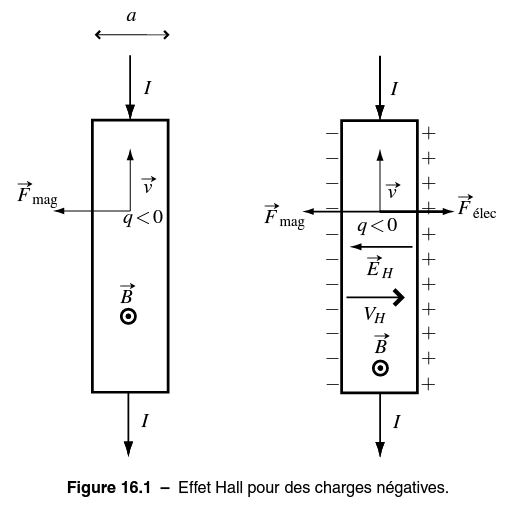
\includegraphics[scale = 0.4]{effet_hall.png}
%	\label{fig:effet_hall.png}
%\end{center}
%\end{figure}

\textcolor{red}{Projeter les calculs qui suivent, ou tout du moins une partie.}

\subsubsection{Bilan des forces}

Une différence de potentiel longitudinale (et donc un champ électrique longitudinal $E_x$) entraîne l'établissement d'une densité volumique de courant $J_x$ (intensité $I$). Lorsqu'on applique le champ magnétique, les électrons sont déviés sous l'effet de la force magnétique $\bold{F}_m = q\bold{v}\times\bold{B}$ : il s'ensuit une accumulation de charge sur les bords du ruban. De cette accumulation naît un champ électrique transverse qui s'oppose à la déviation des électrons. Tant qu'il n'y a pas suffisamment d'électrons déviés, la force électrique $\bold{F}_e = q\bold{E}$ ne suffit pas à contrebalancer la force magnétique et le courant continue d'être dévié.\\

Effectuons un bilan des forces sur un élément de volume (de fluide électronique) $d\mathcal{V}$ :
\begin{equation}
	m n \frac{d\bold{v}}{dt}d\mathcal{V} = n q \left(\bold{E} + \bold{v}\times\bold{B}\right) d\mathcal{V} - \frac{n m }{\tau} \bold{v} d\mathcal{V},
\end{equation}
d'où
\begin{equation}
	\frac{d\bold{v}}{dt} = \frac{q}{m}\left(\bold{E} + \bold{v}\times\bold{B}\right) - \frac{\bold{v}}{\tau}.
\end{equation}

%\begin{equation}
%	m\frac{dv_x}{dt} = qE_x + qv_yB_z - \frac{m}{\tau}v_x
%\end{equation}
%
%\begin{equation}
%	m\frac{dv_y}{dt} = qE_y - qv_xB_z - \frac{m}{\tau}v_y
%\end{equation}

\subsubsection{Régime permanent}

Le régime transitoire prend fin lorsque la force magnétique est compensée par la force électrique transverse. Les électrons ne sont alors plus déviés selon la direction $y$ et on atteint un régime permanent. L'équation du mouvement devient
\begin{equation}
	\bold{0} = \frac{q}{m}\left(\bold{E} + \bold{v}\times\bold{B}\right) - \frac{\bold{v}}{\tau}.
\end{equation}

Introduisons la densité de courant $\bold{J} = n q \bold{v}$ :
\begin{equation}
	\frac{\bold{J}}{nq\tau} = \frac{q}{m}\left(\bold{E} + \frac{\bold{J}}{nq}\times\bold{B}\right),
\end{equation}
d'où 
\begin{equation}
	\bold{J} = \frac{nq^2\tau}{m}\left( \bold{E} + \frac{\bold{J}}{nq}\times\bold{B}\right),
\end{equation}
d'où
\begin{equation}
	\bold{E} = \frac{\bold{J}}{\sigma_0} - \frac{\bold{J}}{nq}\times\bold{B} = \bold{E}_\parallel + \bold{E}_\perp,
\end{equation}
avec $\sigma_0 = \frac{ne^2\tau}{m}$ et avec
\begin{equation}
	\bold{E}_\parallel = \frac{\bold{J}}{\sigma_0} \quad\text{et}\quad \bold{E}_\perp = - \frac{\bold{J}}{nq}\times\bold{B}.\\
\end{equation}

Le champ électrique possède une composante parallèle à $\bold{J}$, et chose nouvelle, \textbf{une composante perpendiculaire à $\bold{J}$ !} : il n'est donc plus colinéaire à $\bold{J}$ et la loi d'Ohm locale a une forme tensorielle :
\begin{equation}
	\bold{J} = \left[\bold{\sigma}\right]\bold{E},
\end{equation}
où $\left[\bold{\sigma}\right]$ est le tenseur de conductivité. La composante $J_x$ de la densité de courant s'écrit alors
\begin{equation}
	J_x = \sigma_{xx} E_x + \sigma_{xy} E_y.\\
\end{equation}

Comme sur le schéma, nous allons nous placer en géométrie allongée, dite \textbf{géométrie de Hall} : soit un ruban de largeur $\ell$, de longueur $L$ et d'épaisseur $h$. Le conducteur est placé dans le vide, la densité de courant étant tangente à la surface du conducteur on a 
\begin{equation}
	\bold{J} = J_x\bold{e}_x,
\end{equation}
d'où
\begin{equation}
	E_\parallel = E_x = \frac{J_x}{\sigma_0} \quad\text{et}\quad E_\perp = - \frac{J_x B_z}{nq} \bold{e}_x\times\bold{e}_z  = \underbrace{\frac{J_x B_z}{nq}}_{E_y}\bold{e}_y.
\end{equation}

Dans cette géométrie, on définit le \textbf{champ électrique de Hall} (champ électrique transverse)
\begin{equation}
	E_H \equiv E_\perp = \frac{J_x B_z}{nq},
\end{equation}
d'où
\begin{equation}
	\frac{E_H}{J_xB_z} = \frac{1}{nq} \equiv R_H,
\end{equation}
où $R_H$ est la \textbf{constante de Hall}.\\

Sa mesure est doublement intéressante :
\begin{itemize}
	\item son signe nous renseigne sur le \textcolor{red}{signe de la charge des porteurs},
	\item sa valeur nous permet de \textcolor{red}{remonter à la densité volumique de porteurs}.
\end{itemize}

%\begin{equation}
%	qE_x = \frac{m}{\tau}v_x \quad\text{et}\quad E_y = v_xB_z.
%\end{equation}
%En multipliant par $-en$ pour faire apparaître $J_x$ et $J_y$
%\begin{equation}
%	\frac{E_x}{J_x} = \frac{1}{\sigma}\quad\text{et}\quad \frac{E_y}{J_xB_z} = \frac{1}{nq}
%\end{equation}
%
%On définit les quantités
%\begin{equation}
%	\boxed{\frac{E_x}{J_x} = \rho_t}\quad\textbf{magnétorésistance transverse},
%\end{equation}
%\begin{equation}
%	\boxed{\frac{E_y}{J_xB_z} \equiv R_H}\quad\textbf{constante de Hall},
%\end{equation}
%et
%\begin{equation}
%	U_H = E_y a,
%\end{equation}

La différence de potentiel entre les points A$+$ et A$-$, liée au champ électrique de Hall, est appelée \textbf{tension de Hall} :\\
\begin{equation}
	V(A+) - V(A-) \equiv U_H = \int_A^B \bold{E}\cdot\bold{dr} = E_H \ell,
\end{equation}
où $b$ est la largeur du ruban conducteur. On peut l'\textbf{exprimer en fonction des paramètres expérimentaux} :
\begin{equation}
	U_H = E_H \ell = \frac{J_x B_z}{nq}\ell = \frac{I}{Snq}B_z \ell = \frac{I B_z}{q n h} = R_H \frac{I B_z}{h},
\end{equation}
si $S = \ell h$ est la section du ruban traversée par le courant d'intensité $I$.\\

D'un point de vue pratique, l'effet Hall a de nombreuses applications : l'une d'elles est la mesure de champ magnétique. Si on connaît bien les caractéristiques physiques et géométriques d'un matériau conducteur, et qu'on travaille à courant constant, la tension de Hall est directement l'image du champ magnétique dans lequel le matériau est plongé.\\

\subsubsection{L'effet Hall pour caractériser un matériau : cas du germanium dopé n}

Outre servir à mesurer un champ magnétique, comme dans un teslamètre, l'effet Hall peut nous servir à caractériser les propriétés de conduction électrique d'un matériau. Pour cela, on doit tracer la courbe $U_H = f(B)$ à courant $I$ constant. Le modèle de Drude prévoit une \textbf{relation linéaire} entre ces deux grandeurs :
\begin{equation}
	U_H = a B,
\end{equation}
où le coefficient de proportionnalité $a$ peut être interprété comme
\begin{equation}
	\boxed{a = \frac{I}{q n h} = v \ell = \mu U \frac{\ell}{L}},
\end{equation}
où $U$ est la tension longitudinale aux bornes du conducteur. Ainsi, \textbf{l'effet Hall nous permet de remonter à toutes les quantités clés intervenant dans le modèle de Drude}, notamment la mobilité $\mu$ \textbf{et par conséquent au temps de relaxation $\tau$}.\\ 

\textit{Démonstration :}
\begin{itemize}
	\item \textcolor{blue}{mesure de v}
	\begin{equation}
		J_x = nqv \quad\text{donc}\quad U_H = \frac{nqvB_z\ell}{nq} = v\ell B_z,
	\end{equation}
	d'où
	\begin{equation}
		\boxed{a = v\ell}.
	\end{equation}
	\item \textcolor{blue}{mesure de $\mu$}
	\begin{equation}
		J_x = n q \mu E_x = n q \mu \frac{U}{L},
	\end{equation}
	d'où
	\begin{equation}
		\frac{n q U_H}{B_z \ell} = n q \mu \frac{U}{L}, \quad\text{donc}\quad U_H = \mu \frac{U}{L} B_z
	\end{equation}
	d'où
	\begin{equation}
		\boxed{a = \frac{\mu U \ell}{L}}
	\end{equation}
\end{itemize}

Le terme $\bold{J}\times\bold{B}$ responsable de la tension de Hall est très faible dans les métaux (la tension est de l'ordre du $\mu V$. Nous allons donc réaliser cette étude sur un semi-conducteur, du \textbf{germanium dopé N}.\\

Nous avons vu qu'un semi-conducteur portait deux types de charges, des électrons et des trous. Dans le cas d'un \textbf{semi-conducteur intrinsèque}, il y a autant d'électrons que de trous : ces semi-conducteurs conduisent assez mal l'électricité. Si on souhaite améliorer leurs performances, il faut ajouter des atomes donneurs d'électrons (on parle de \textbf{dopage N}) ou accepteurs d'électrons (et donc donneurs de trous, on parle de \textbf{dopage P}) : le semi-conducteur est alors qualifié d'\textbf{extrinsèque} et on considère que le remplacement d'un atome d'origine sur un million par un atome dopant suffit à ce que la conduction à température ambiante ne dépende que des électrons ou des trous créés par les atomes étrangers.\\

On utilise ici un cristal de Germanium, \textbf{dopé N} . On pourra considérer que seuls les électrons sont responsables de la conductivité électrique. On se propose de mesurer $n$, $\mu$ et $v$, puis d'en déduire le temps caractéristique correspondant $\tau$. Pour cela, on place le cristal de germanium dans un \textbf{électroaimant} générant un champ magnétique de quelques dizaines de mT. On mesure directement la tension de Hall $U_H$, la tension longitudinale $U$, le courant $I$ et le champ magnétique $B$ produit par l'électroaimant. On travaille à courant constant, et donc à $U$ constante.\\

Le dopage du cristal nous permet d'utiliser les relations définies plus haut.\\

Il y a beaucoup moins de porteurs par maille dans un semi-conducteur que dans un métal comme le cuivre, pour un pas de réseau cristallin de taille comparable.

\newpage
\section{Au-delà du modèle de Drude}

\subsection{Limites du modèle de Drude}

Bien que simple, le modèle de Drude peut fournir des renseignements précieux sur un matériau conducteur en première approche : c'est pour cela qu'\textbf{il est encore utilisé aujourd'hui, moyen pratique et rapide pour obtenir une estimation grossière} de certaines propriétés du matériau. Il est également capable de restituer la loi d'Ohm à partir de considérations microscopiques. Ce modèle n'est cependant pas parfait.\\

\subsubsection{Incapacité à distinguer un isolant d'un conducteur}

\textbf{Le modèle de Drude est incapable de rendre compte des différences entre métaux, semi-conducteurs et isolants} en dehors d'une basique comparaison de leurs conductivités électriques respectives :
\begin{itemize}
	\item que sont ces "trous" qui semblent conduire l'électricité dans les semi-conducteurs ?
	\item pour certains métaux, la constante de Hall est positive (effet Hall anormal), impliquant un courant de charges positives au sein d'un métal.
	\item on observe des différences de comportement importantes entre conducteurs et semi-conducteurs : la \textbf{résistance d'un métal croît linéairement avec la température}, alors que \textbf{celle d'un semi-conducteur intrinsèque décroit de façon exponentielle avec $T$} !\\
\end{itemize}

\subsubsection{Nécessité de la mécanique quantique}

C'est la \textbf{mécanique quantique} qui nous permet aujourd'hui de construire un modèle plus respectueux des résultats expérimentaux. Montrons pourquoi l'utilisation de la mécanique quantique est indispensable à une bonne description du comportement des électrons dans un solide.\\

\subsubsection{L'hypothèse des électrons libres est mauvaise}

Durant la première moitié du vingtième siècle étaient posées les premières fondations de ce qui deviendrait quelques décennies plus tard la mécanique quantique :
\begin{itemize}
	\item 1913 : les Bragg, père et fils, sondent la matière solide grâce aux rayons X et mettent en évidence la répartition périodique des atomes ou ions à l'échelle microscopique. Les ions dans les métaux ne sont donc pas répartis au hasard, mais de façon régulière, avec une périodicité mesurable, de l'ordre de quelques Angström ($10^{-10}$ m).\\
	
	\item 1923 : Louis de Broglie établit le \textbf{concept de dualité onde-corpuscule} dont nous avons déjà parlé lors d'une leçon précédente.\\
\end{itemize}

La mécanique quantique prévoit que les électrons ne peuvent pas avoir n'importe quelle énergie : $E$ est quantifiée et il existe donc un ensemble de niveaux d'énergie discrets $E_i$.\\

Les électrons sont des \textbf{fermions} (particules de spin demi entier), ils obéissent donc à la statistique de Fermi-Dirac
\begin{equation}
	f_i = \frac{1}{\text{exp}\left(\frac{E_i - \mu}{k_B T} \right)+1}, \quad\text{où }\mu\text{ est le potentiel chimique du gaz,}
\end{equation} 
qui est \textbf{très différente de celle de Maxwell-Boltzmann à température ambiante et pour des densités de l'ordre de $10^{28} \text{m}^{-3}$} électrons (cas des métaux) : selon cette statistique, l'\textbf{énergie moyenne d'un électron est de quelques eV} alors que l'énergie moyenne prédite par la théorie de Maxwell-Boltzmann est plutôt \textbf{de l'ordre de $k_B T \simeq 10^{-2}$ eV} ; la différence est de taille.\\

On rappelle que l'énergie du dernier état occupé est nommée \textbf{énergie de Fermi} $E_F$, à laquelle on associe une \textbf{vitesse de Fermi} $v_F$, telle que
\begin{equation}
	E_F = \frac{1}{2}m v_F^2.
\end{equation}
Cette vitesse joue dans la théorie d'un gaz de Fermi un rôle similaire à celle de la vitesse quadratique moyenne du gaz classique. A l'état fondamental, elle est de l'ordre de $v_F \simeq 10^6$ m/s (\textbf{et la température est nulle !}).\\

Calculons maintenant la longueur d'onde de De Broglie des électrons :
\begin{equation}
	\lambda = \frac{h}{m v_F} \simeq 7\times 10^{-10} \text{m},
\end{equation}
soit quelques Angström, comparable à la périodicité spatiale des ions dans un métal. Il en résulte que le comportement ondulatoire des électrons ne peut pas être négligé :
\begin{itemize}
	\item cela confirme bien la nécessité de remplacer la statistique de Maxwell-Boltzmann par celle de Fermi-Dirac;
	\item un traitement quantique complet du problème est nécessaire, au-delà du seul changement de la  statistique;
	\item l'approximation des électrons libres ne tient pas : les ions sont des particules chargées, générant un potentiel électrique inhomogène dont la longueur caractéristique est comparable à $a$ et donc à la longueur d'onde de De Broglie des électrons.
\end{itemize}

\subsection{Quelques résultats de la théorie des bandes}

\textcolor{red}{Expliquer avec un diagramme représentant les bandes et le gap dans le cas d'un isolant et d'un métal. Deuxième diapo avec le cas des semi-conducteurs et valeur des gaps}\\

Nous allons présenter ici quelques résultats de la théorie des bandes qui nous permettront de répondre aux interrogations suscitées par l'expérience, auxquelles le modèle de Drude ne peut répondre. La liste sera bien entendu non exhaustive.\\

Dans un solide, sous l'effet combiné de la périodicité du potentiel et des interactions, les niveaux d'énergie électroniques se rassemblent et forment des \textbf{bandes d'énergie} à l'intérieur desquelles la différence entre deux niveaux successifs est très faible devant la différence d'énergie entre le premier et le dernier niveau de la bande : les niveaux forment un quasi-continuum. En revanche, deux bandes sont séparées par un ensemble de niveaux d'énergie interdits : on parle de \textbf{bande interdite}. La largeur de cette bande est une énergie, qu'on appelle \textbf{énergie de bande interdite, ou gap} $E_g$\\ 

La \textbf{dernière bande entièrement occupée} est appelée \textbf{bande de valence} : les électrons qui s'y trouvent participent à des \textbf{liaisons covalentes}, bien localisées. La dernière bande partiellement occupée ou la première bande inoccupée est appelée \textbf{bande de conduction}. Les électrons qui s'y trouvent participent aux \textbf{liaisons métalliques} délocalisées, permettant aux électrons de migrer pour conduire l'électricité.\\

\subsubsection{Peuplement des bandes d'énergie}

\'A basse température, seuls les niveaux d'énergie inférieurs au potentiel chimique sont occupés. La \textbf{position du potentiel chimique dans la structure de bandes} des solides permet alors de mettre en évidence leur caractère conducteur ou isolant :
\begin{itemize}
	\item si le potentiel chimique se trouve dans une bande interdite, tous les électrons sont dans la bande de valence et il leur est pratiquement impossible d'accéder à la bande de conduction : il faudrait appliquer une différence de potentiel telle que $eV >> E_g$.\\
	\item si le potentiel chimique se trouve dans une bande permise, il suffit d'un faible apport d'énergie pour que des électrons atteignent des niveaux d'énergie supérieurs et se mettent à conduire l'électricité.\\
\end{itemize}

Ainsi, dans un métal ou un isolant, \textbf{l'influence de $T$ sur le peuplement des niveaux énergétiques des bandes est sans effet notable} : on a toujours à peu près le même nombre d'électrons dans une bande donnée. \textbf{Il existe toutefois des matériaux pour lesquels l'énergie de bande interdite $E_g$ est suffisamment faible} (inférieure ou proche de 1 eV) pour que \textbf{l'agitation thermique ($k_B T$ de l'ordre de quelques dizaines de meV) suffise à promouvoir un électron} de la bande de valence vers la bande de conduction. Ces électrons sont alors libres de conduire l'électricité lorsqu'on applique un champ électrique. La promotion d'un électron vers un niveau d'énergie supérieur implique l'\textbf{apparition d'un "trou" dans la bande de valence} (\textbf{on dit qu'il y a création d'une paire électron-trou}) que d'autres électrons de cette bande peuvent alors occuper. Le déplacement de ces électrons sous l'effet d'un champ électrique peut être considéré comme celui d'un trou en sens inverse, et donc comme celui d'une particule de charge positive. On a conduction d'électrons dans la bande de conduction et conduction de trous dans la bande de valence.\\

\subsubsection{Influence de la température sur la résistivité d'un solide}

Évaluons le libre parcours moyen des électrons à l'aide de la vitesse de Fermi et du temps de relaxation
\begin{equation}
	\ell \equiv \frac{v_F}{\tau} \simeq 10^6 \times 10^{-14} \simeq 10^{-8} \text{à} 10^{-9} \text{m}.
\end{equation}
Ce résultat est nettement supérieur au pas du réseau cristallin, ce qui semble invalider l'hypothèse de Drude selon laquelle les collisions électron ion seraient responsables de la résistivité d'un solide. En réalité, la résistivité d'un métal est imputable aux imperfections du réseau : défauts de structure, impuretés, agitation thermique des ions (et donc vibrations du réseau).\\

Puisque la conductivité dépend de la mobilité et de la densité des porteurs, et que la mobilité, proportionnelle au libre parcours moyen, décroît avec la température, c'est la dépendance du nombre de porteurs en fonction de la température \textbf{(dépendance absente dans le modèle de Drude)} qui va nous permettre de distinguer les conducteurs des semi-conducteurs :
\begin{itemize}
	\item les électrons de conduction d'un métal sont, à température nulle, dans une bande de conduction partiellement vide. Une augmentation de température fera migrer ces électrons vers des niveaux d'énergie libres de la bande de conduction mais n'aura quasiment aucune influence sur le nombre d'électrons contenus dans la bande de conduction. \textbf{La densité de porteurs d'un métal est donc indépendante de la température}. C'est la dépendance de la mobilité vis à vis d $T$ qui explique donc celle de la résistivité : plus $T$ augmente, plus la mobilité des charges diminue du fait de l'augmentation des vibrations du réseau.\\
	\item dans un semi-conducteur intrinsèque, le nombre de paires électron-trou augmente exponentiellement avec la température. Cette augmentation masque totalement la perte de mobilité des porteurs de charge. La résistivité d'un semi-conducteur diminue donc avec la température.
\end{itemize}

\newpage
\section*{Conclusion}

Pour aller davantage dans le détail, il faudrait aller plus loin dans la théorie des solides. Retenons que la circulation d'un courant électrique dans un conducteur provoque un échauffement de celui-ci, par effet Joule. Ceci est problématique lorsqu'on souhaite transporter de l'électricité sur de très longues distances (à travers un pays, par exemple) ou des courants de très haute intensité. Ces derniers sont nécessaires dans divers types d'application, notamment la génération de champs magnétiques intenses (par exemple $B \simeq 11.8 T$ dans le projet ITER, nécessitant un courant d'intensité $I = 68 000 \;A$).\\

Lorsqu'on refroidit certains types de matériaux sous une température critique $T_c$, par exemple le niobium titane ($T_c \simeq 10 K$), ils deviennent supraconducteurs :
\begin{itemize}
	\item la résistivité est nulle,
	\item le matériau devient un diamagnétique parfait : le champ $\bold{B}$ ne pénètre plus dans le matériau. 
\end{itemize}
La réalisation de supraconducteurs à haute température critique est un enjeu physique majeur, dont les applications seraient d'une importance considérable. En attendant, procédés de cryogénie indispensables.
\end{document}